

\documentclass[12pt,letterpaper,notitlepage]{report}

\usepackage{graphicx}

\usepackage{natbib}

\usepackage[T1]{fontenc}

\usepackage{ucs}

\usepackage[utf8x]{inputenc}

\usepackage[spanish]{babel}

\usepackage{helvet}

\usepackage{url}

\usepackage{sectsty}

\usepackage[small,sf]{caption}

\setlength{\oddsidemargin}{0. true cm}

\setlength{\evensidemargin}{0. true cm}

\setlength{\protect\textwidth}{16.5 true cm}

\setlength{\topmargin}{0.0 true cm}

\setlength{\textheight}{20 true cm}

\newcommand{\ie}{{\em   i.e.   }}    \newcommand{\eg}{{\em  e.g.    }}
\newcommand{\txh}{\textheight}

\newcommand{\txw}{\textwidth}

\newcommand{\scrsz}{\scriptsize}

\newcommand{\mc}[3]{\multicolumn{#1}{#2}{#3}}

\newcommand{\Cpp}{{\bfseries C++}}



% Some commands to handle linespacing

\newlength{\spacing} \setlength{\spacing}{\baselineskip}

\newcommand{\nspace}[1]{\setlength{\baselineskip}{#1\spacing}}
\newenvironment{linespacing}[1]{\nspace{#1}}{}

\newcommand{\SM}{{\bfseries\emph {SumCfsmplx}}}

\allsectionsfont{\sffamily}

\bibliographystyle{apalike}

\title{Manual de usuario del Paquete\\ ``imageServer''.}

\author{Dr. Arturo Espinosa Romero\\Dr. Carlos Brito Loeza\\Dr. Ricardo Legarda Saenz}

\date{}

\begin{document}

 {\sffamily

 \maketitle

\begin{linespacing}{1.5}

\section{Introducción.}

El objetivo de este paquete es  el de proporcionar una herramienta que
permita  la distribución de imágenes capturadas desde una cámara a múltiples usuarios que se encuentran distribuidos en lugares diferentes, a través de internet. Las imágenes transmitidas pueden sufrir previa a su transmisión transformaciones lineales de rectificación y enmascaramiento, así como proveer mecanismos que faciliten el el análisis temporal de las imágenes, esto es considerar transformaciones que consideren el flujo de imágenes y no sólo imágenes aisladas. 

El paquete imageServer es importante en  en ámbitos de investigación aplicada así como la docencia, en donde es necesario que múltales actores, puedan acceder de manera simultanea a imágenes capturadas en un sitio. En particular este programa se aplica en dos actividades principalmente: en la captura y análisis de imágenes aéreas, y en la teleoperación de robots móviles en laboratorio. 

La organización de  este documento es como  sigue: primero describimos
las partes que constituyen el paquete computacional, a continuación se
da una guía rápida de uso, para después presentar resultados obtenidos.

Este  paquete fue  desarrollado como  parte  de la  segunda etapa  del
proyecto "Sistema Automático de Bajo  Costo para la Captura y Análisis
de Imágenes  Aéreas" que se  está realizando como  parte de la  red de
Investigación  Conjunta para  Solución  de  Problemas en  Adquisición,
Procesamiento  de Señales  y  Control Automáticos  de Dispositivos  de
Sensado Remoto. apoyado por PRODEP.

\section{Descripción.}

El  paquete se construyo utilizando estructuras de datos y  métodos de la biblioteca openCV~\citep{opencv_library} principalmente y esta compuesto por un conjunto de módulos que se detallan a continuación:

\begin{itemize}

\item {\bfseries ImageServer:} Este modulo consiste en un conjunto de biblioteca de funciones que permiten construir un servidor capaz de atender múltiples clientes de manera concurrente, y atender solicitudes de éstos para enviar imágenes. El programa crea un \emph {stream socket}, que se asocia a una dirección IP(v4). Cuando un cliente se conecta se crea una nueva hebra para atender dicho cliente, y permitirle acceder a imágenes capturadas.

\item {\bfseries Camera} Este módulo captura imágenes de un dispositivos de captura y las almacena en una \emph {buffer} (cola circular). Provee mecanismos de sincronización para controlar el acceso a los elementos de la cola.

\item {\bfseries imgServer} Es el programa donde los diferentes componente necesarios para construir el servidor de imágenes se combinan. El programa recibe como parámetros las dirección IP(v4) y número de puerto que se va a asociar al servidor, y un archivo que contiene una mascara que se aplicara a las imágenes capturadas. Cada imagen capturada por el usuario se le somete a dos transformaciones geométricas. La primera sirve para rectificar la imagen, en caso necesario, y la segunda para ajustar el tamaño de la máscara al tamaño de la imagen capturada. El modelo de rectificación se calcula a partir de información que provee el usuario, seleccionando la región planar de la escena a observar. 

\item {\bfseries Client} El cliente consiste de dos principales miembros. Una clase que provee de métodos que facilitan la conexión con el servidor de imágenes, así como la descarga de imágenes de éste, y dos programas de ejemplo una escrito en C++, y el otro un \emph {script} de python que sirven como guía para desarrollar programas mas complejos, y el uso del servicio en otros ámbitos. 

\end{itemize}

\section{Guía de uso.}
 
El  código esta  preparado para  ser compilado  en una  computadora que
tenga como  sistema operativo alguna  variante de Unix (\emph  {e.g. }
Linux, MacOS),  aunque es posible  también compilarlo y  utilizarlo en
otras plataformas.

La interacción con el programa  se hace invocándolo desde una emulador
de terminal.  Primero que hay que  ubicarse en el directorio  en donde
está el  código y  compilarlo utilizando el  programa make\footnote{se
asume que en  el sistema está instalado las  bibliotecas de desarrollo
de \textbf{openCV}}.

\smallskip


\begin{verbatim}
$ make
\end{verbatim}


\smallskip

Un vez  que se  ha compilado  el código se  puede invocar  como sigue:
{\small
\begin{verbatim} 
$ ./imgServer CamId IPAddres Puerto ArchivoMascara
\end{verbatim} }

El primero parámetro es el identificador de cámara que se va a utilizar (un numero entero, el segundo parámetro es una direccion IP(v4), el tercer parámetro es el numero de puerto y por último el último parámetro es el archivo que contiene la imagen que se va a usar como máscara. La máscara opera como sigue: en aquellos pixeles de la máscara que son diferentes a RGB[255,255,255] (color blanco), el pixel correspondiente de la imagen se sustituye por el valor de la máscara. De caso contrario, el valor original del pixel, se preserva.

Una vez que se invoca, el programa abre una ventana en donde se muestra la escena que esta siendo capturada por la cámara. Aqui el usuario puede seleccionar las cuatro esquinas de un paralelogramo contenido en algun plano de la imagen, con el fin de calcular la rectificación, en dado caso que ésto no sea necesario, solo hay que seleccionar las cuatro esquinas de la imagen, comenzado desde la esquina superior izquierda procediendo a favor de las manecillas del reloj.

Una vez que se ha hecho, en la consola desde donde se invocó el programa se muestra las matrices de transformación calculadas, y el servidor permanece en ejecución aceptando conexiones de los clientes del sistema. En la figura\ref{fig:imgConsola} se muestra una captura de dicha consola así como la imagen en donde se muestran las cuatro esquinas capturadas.
 
\begin{figure}[htbp!]
  \centering
  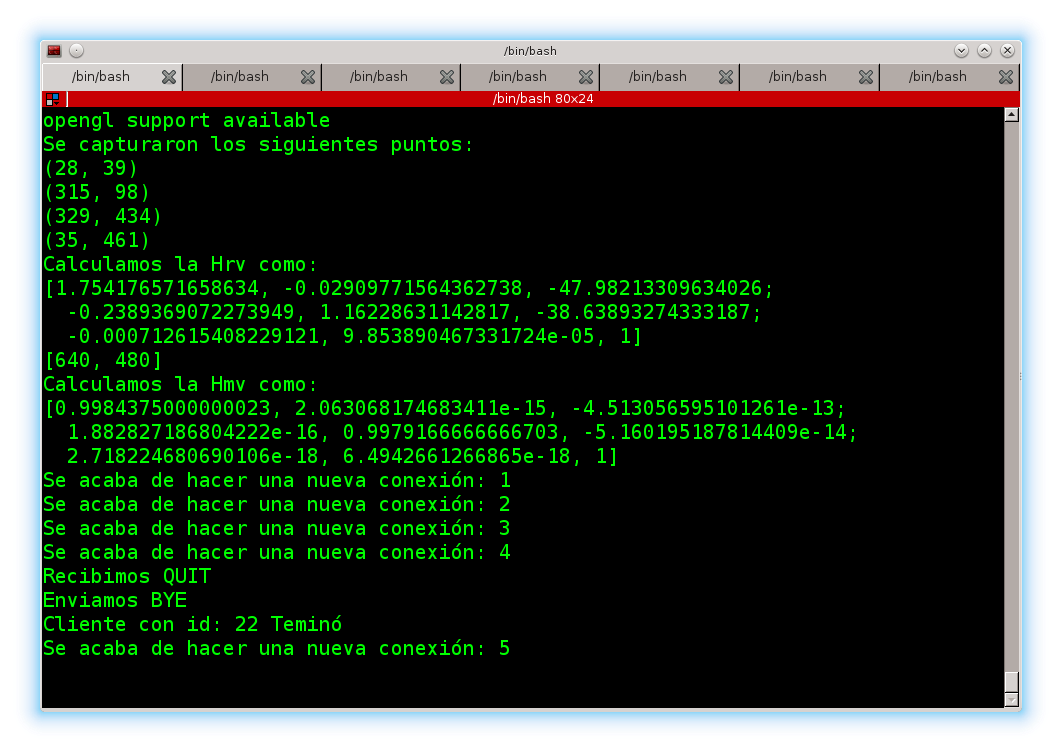
\includegraphics[width=\textwidth]{imagenes/imgServerConsole.png}\\
  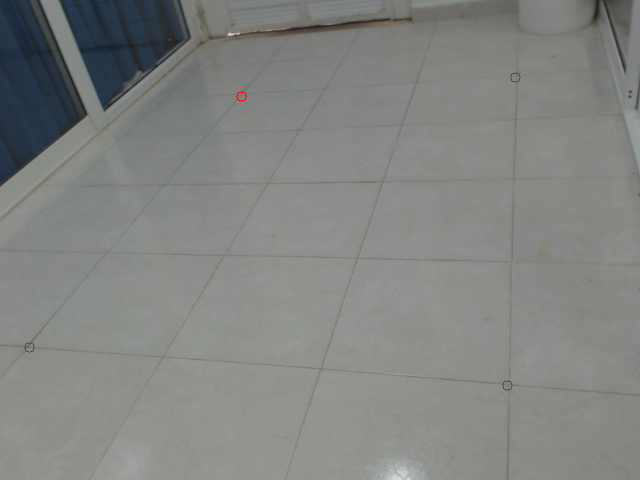
\includegraphics[width=\textwidth]{imagenes/inImage1A.png}\\
  \caption{Invocación del servidor desde una consola, y la imagen de donde el usuario selecciona el paralelogramo en un plano de la escena, para calcular la rectificación.}
  \label{fig:imgConsola}
\end{figure}

Una vez que se ejecuta el servidor, desde cualquier otra computadora que pueda acceder al servidor puede ejecutarse un archivo cliente que obtenga las imagenes. En nuestro caso utilizamos el programa \verb|testClient|:

  {\small
\begin{verbatim} 
$ ./testClient IPAddres Puerto
\end{verbatim} }

El primero parámetro es una direccion IP(v4), y el segundo parámetro es el numero de puerto. Al ejecutarse, el programa abre una ventana y muestra las imagenes que recibe del servidor. Ejemplos de las imagenes que recibe se muestran en la figura~\ref{fig:testClient}. Dichos ejemplos muestra un ejemplo del sistema en una operación de teleoperación de robots móviles. 

\begin{figure}[htbp!]
  \centering
  \begin{tabular}{cc}
    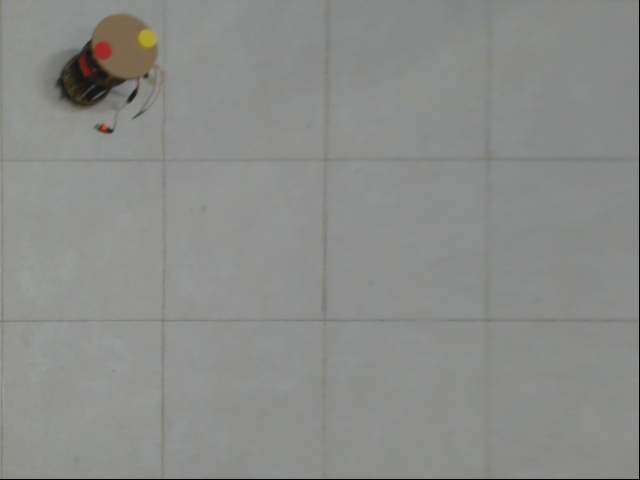
\includegraphics[width=0.47\textwidth]{imagenes/outImage_00121_A.png}&
    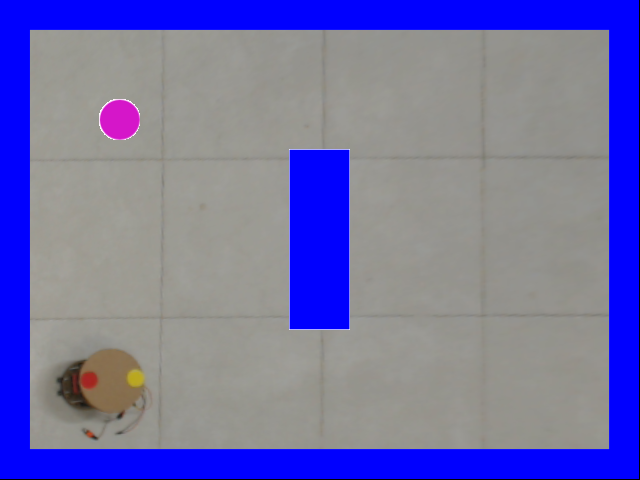
\includegraphics[width=0.47\textwidth]{imagenes/outImage_00151.png}\\
    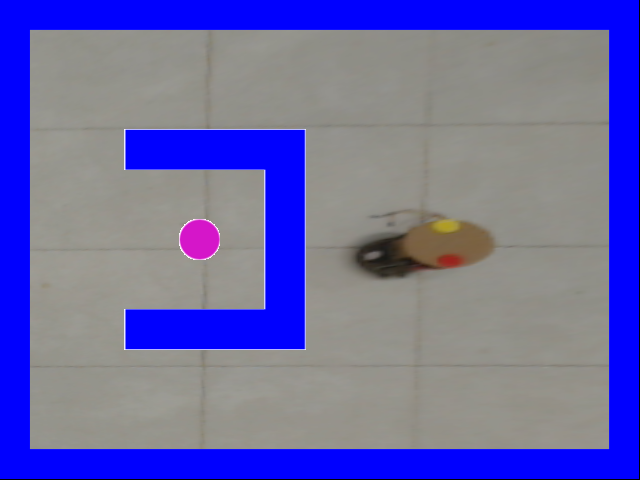
\includegraphics[width=0.47\textwidth]{imagenes/outImage_00766.png}&
    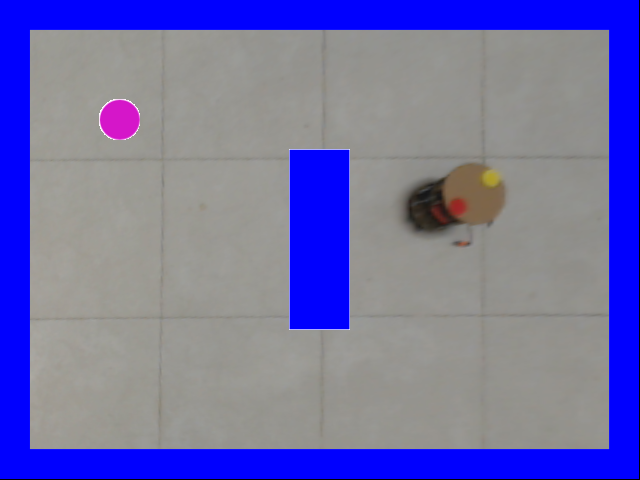
\includegraphics[width=0.47\textwidth]{imagenes/outImage_00796.png}\\
  \end{tabular}
  \caption{Imagenes mostradas por el programa testClient. En la esquina superior izquiera se muestra una imagen capturada sin utilizar ninguna máscara, y las tres siguientes imagenes muestran imágenes con algun tipo de máscara añadidio.}
  \label{fig:testClient}
\end{figure}


\end{linespacing}

\bibliography{biblio}

}
\end{document}

%%% Local Variables: %%% mode: latex %%% TeX-master: t %%% End:
